\documentclass[10pt, aspectratio=169]{beamer}

% Pakete
\usepackage[utf8]{inputenc}
\usepackage[T1]{fontenc}
\usepackage[ngerman]{babel}
\usepackage{graphicx}
\usepackage{hyperref}
\usepackage{xcolor}

% --- DESIGN: "Website im Aufbau / Raw HTML" ---
\usetheme{default}         % Kein Theme, keine Boxen, keine Leisten
\usefonttheme{serif}       % Klassische Serifenschrift (wie Times New Roman im Browser)
\setbeamertemplate{navigation symbols}{} % Keine Navigationssymbole

% Klassische "Web-Link" Farbe (Blau) definieren
\definecolor{webblue}{HTML}{0000EE}
\hypersetup{
    colorlinks=true,
    linkcolor=webblue,
    urlcolor=webblue,
    citecolor=webblue
}

% Titel etwas "roher" gestalten (fett und linksbündig)
\setbeamertemplate{frametitle}{\bfseries\insertframetitle\par\vspace{0.2cm}\hrule}

% Metadaten
\title[Lineare Anamorphose]{Lineare Anamorphose und ihre mathematischen Grundlagen}
\subtitle{Von der Renaissance-Perspektive zur projektiven Geometrie}
\author{Daniel Stumpp}
\institute[Mathematik]{Geschichte der Mathematik}
\date{9. Februar 2026}

\begin{document}

% -------------------------------------------------------------------------
% Folie 1: Titelseite
% -------------------------------------------------------------------------
\begin{frame}
    \titlepage
    \centering
\end{frame}

% -------------------------------------------------------------------------
% Folie 2: Definition
% -------------------------------------------------------------------------
\begin{frame}{Definition \& Prinzip}
    \begin{columns}[c]
        % Linke Spalte: Text
        \column{0.6\textwidth}
        \textbf{Was ist Anamorphose?}
        \begin{itemize}
            \item \textbf{Etymologie:} Griechisch \textit{ana} (zurück/wieder) und \textit{morphe} (Gestalt) $\rightarrow$ „Umformung“
            \item \textbf{Das optische Prinzip:}
            \begin{itemize}
                \item Ein verzerrtes Bild, das nur aus einem \textit{einzigen, fixierten Blickpunkt} in wahren Proportionen erkennbar ist
                \item Gegensatz zur Zentralperspektive: Der Betrachter wird mathematisch diszipliniert
            \end{itemize}
        \end{itemize}

        % Rechte Spalte: Bild
        \column{0.4\textwidth}
        \begin{figure}
            \centering
            % Denke an die verkleinerten Bilder!
            \includegraphics[width=\textwidth, height=0.7\textheight, keepaspectratio]{bild_schema.jpg}
            \caption{Schematische Darstellung: Augenpunkt \& Bildebene.}
        \end{figure}
    \end{columns}
\end{frame}

% -------------------------------------------------------------------------
% Folie 3: Historische Einordnung
% -------------------------------------------------------------------------
\begin{frame}{Historische Einordnung}
    \begin{columns}[c]
        \column{0.6\textwidth}
        \textbf{Ursprung in der Renaissance}
        \begin{itemize}
            \item \textbf{Erfindung:} Leonardo da Vinci (Codex Atlanticus, ca. 1485) fertigte die ersten anamorphotischen Skizzen an
            \item \textbf{Kontext 16. Jahrhundert:}
            \begin{itemize}
                \item Perfektionierung der Zentralperspektive
                \item Anamorphose als „Spielart“: Was passiert, wenn der Fluchtpunkt extrem verschoben wird?
                \item Verschlüsselung von Botschaften
            \end{itemize}
        \end{itemize}

        \column{0.4\textwidth}
        \begin{figure}
            \centering
            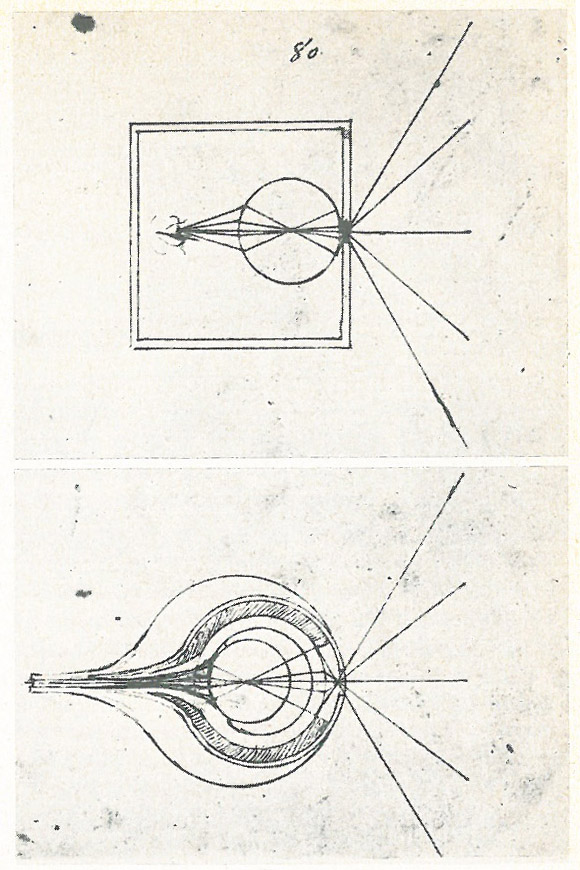
\includegraphics[width=\textwidth, height=0.7\textheight, keepaspectratio]{leonardo_skizze.jpg}
            \caption{Leonardos Skizze eines Auges (Codex Atlanticus).}
        \end{figure}
    \end{columns}
\end{frame}

% -------------------------------------------------------------------------
% Folie 4: Mathematische Kernidee
% -------------------------------------------------------------------------
\begin{frame}{Mathematische Kernidee: Projektive Geometrie}
    \begin{columns}[c]
        \column{0.6\textwidth}
        \textbf{Die Geometrie der Sehstrahlen}
        \begin{itemize}
            \item \textbf{Projektion:} Quadratisches Gitter $\rightarrow$ langgestrecktes Trapez
            \item \textbf{Konstruktion (Niceron):}
            \begin{itemize}
                \item Nutzung von gespannten Fäden als Sehstrahlen
                \item Zwingender Fixpunkt (Guckloch)
            \end{itemize}
            \item \textbf{Nicerons Stuhl:}
            \begin{itemize}
                \item Chaos wird Ordnung nur von einem Punkt aus
            \end{itemize}
        \end{itemize}

        \column{0.4\textwidth}
        \begin{figure}
            \centering
            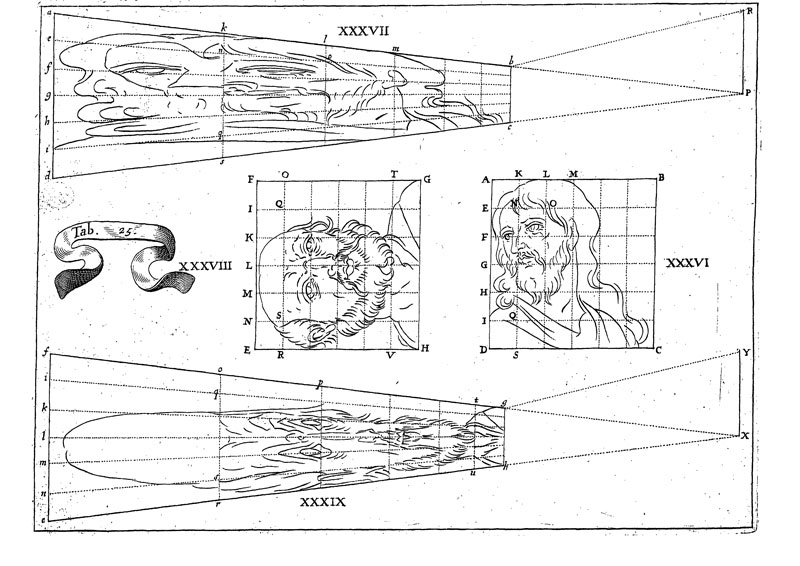
\includegraphics[width=\textwidth, height=0.7\textheight, keepaspectratio]{niceron_stuhl.jpg}
            \caption{Konstruktionsschema (Niceron, 1638).}
        \end{figure}
    \end{columns}
\end{frame}

% -------------------------------------------------------------------------
% Folie 5: Fallbeispiel Holbein
% -------------------------------------------------------------------------
\begin{frame}{Fallbeispiel: Hans Holbein d. J. – „Die Gesandten“ (1533)}
    \begin{columns}[c]
        \column{0.6\textwidth}
        \textbf{Das berühmteste Vexierbild}
        \begin{itemize}
            \item \textbf{Das Phänomen:} Ein amorpher Fleck stört die Darstellung
            \item \textbf{Mathematische Entzerrung:}
            \begin{itemize}
                \item Winkel: Extrem flach von rechts oben
                \item Resultat: Ein \textbf{Totenkopf}
            \end{itemize}
            \item \textbf{Symbolik \& Signatur:}
            \begin{itemize}
                \item \textit{Memento Mori:} Mahnung an die Vergänglichkeit
                \item Wortspiel: „Hol-bein“ $\rightarrow$ „Hohles Bein“ (Knochen)
            \end{itemize}
        \end{itemize}

        \column{0.4\textwidth}
        \begin{figure}
            \centering
            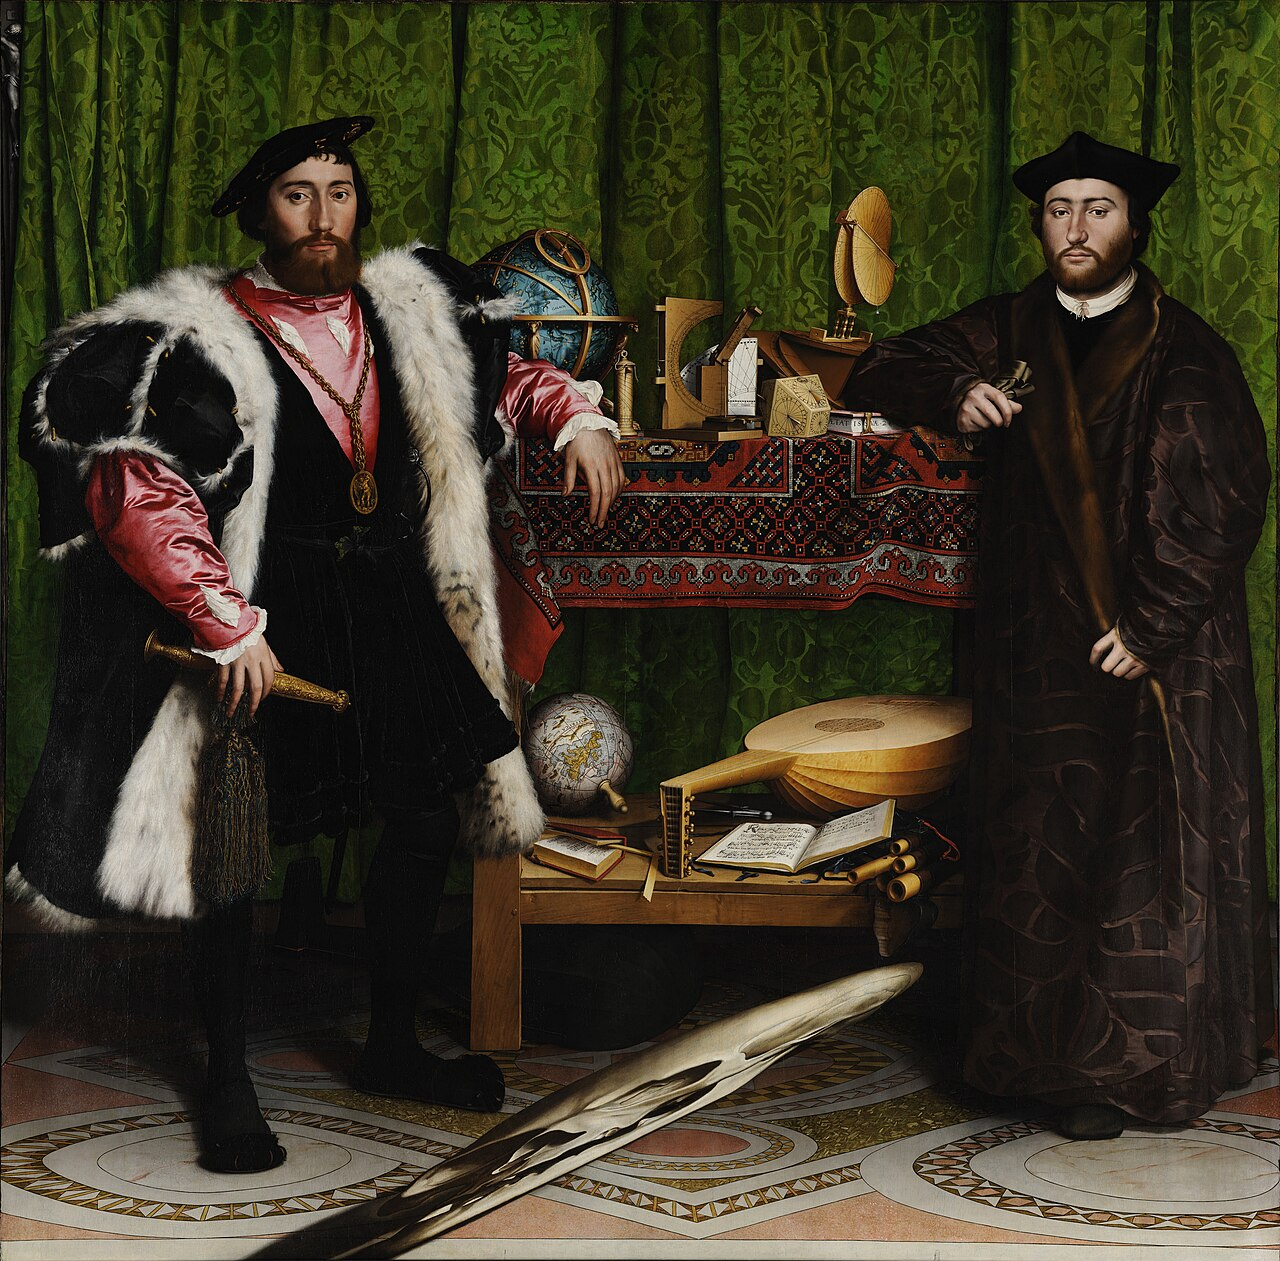
\includegraphics[width=\textwidth, height=0.6\textheight, keepaspectratio]{holbein_skull.jpg}
            \caption{Verzerrter Schädel und Entzerrung.}
        \end{figure}
    \end{columns}
\end{frame}

% -------------------------------------------------------------------------
% Folie 6: Monumentale Anwendung
% -------------------------------------------------------------------------
\begin{frame}{Monumentale Architektur-Anamorphose}
    \begin{columns}[c]
        \column{0.55\textwidth}
        \textbf{Emmanuel Maignan (Rom, 1642)}
        \footnotesize
        \begin{itemize}
            \item \textbf{Ort:} Kloster Trinità dei Monti (17m lang)
            \item \textbf{Der Effekt:}
            \begin{itemize}
                \item Frontal: Landschaft \& Bäume
                \item Seitlich: \textbf{Hl. Franz von Paola}
            \end{itemize}
            \item \textbf{Mathematik:}
            \begin{itemize}
                \item Inverse Perspektive auf Gewölbe
                \item Buch: \textit{Perspectiva horaria}
            \end{itemize}
        \end{itemize}
        
        \column{0.45\textwidth}
        \begin{figure}
            \centering
            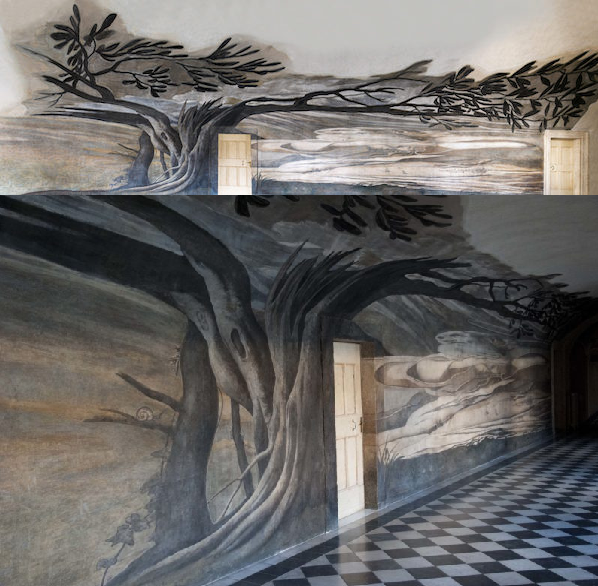
\includegraphics[width=\textwidth, height=0.7\textheight, keepaspectratio]{maignan_fresco.jpg}
            \caption{Landschaft vs. Heiligenfigur.}
        \end{figure}
    \end{columns}
\end{frame}

% -------------------------------------------------------------------------
% Folie 7: Relevanz & Diskussion
% -------------------------------------------------------------------------
\begin{frame}{Relevanz \& Diskussion}
    \textbf{Warum heute noch relevant?}
    \begin{itemize}
        \item \textbf{Street Art:} 3D-Illusionen (Julian Beever)
        \item \textbf{Psychologie:} \textit{Ames-Raum}
        \item \textbf{Verkehr:} Fahrbahnmarkierungen
    \end{itemize}

    \vspace{0.5cm}
    \textbf{Fragen an das Publikum:}
    \begin{enumerate}
        \item Anamorphosen in deinem Alltag?
        \item Unterschied: Analog vs. VR-Verzerrung?
        \item Rolle des aktiven Betrachters?
    \end{enumerate}
\end{frame}

% -------------------------------------------------------------------------
% Quellen
% -------------------------------------------------------------------------
\begin{frame}[allowframebreaks]{Wissenschaftliche Quellen}
    \begin{thebibliography}{10}
        \bibitem{Niceron1638} Niceron, J.-F. \textit{La perspective curieuse}. Paris, 1638.
        \bibitem{Baltrusaitis1984} Baltrušaitis, J. \textit{Anamorphoses}. Flammarion, 1984.
        \bibitem{Maignan1648} Maignan, E. \textit{Perspectiva horaria}. Rom, 1648.
        \bibitem{Hunt2000} Hunt, J.L. et al. \textit{Anamorphic Images}. Am. J. Phys, 68, 2000.
    \end{thebibliography}
\end{frame}

\end{document}